\documentclass{beamer}
\usepackage{tikz,pgfplots}
\pgfplotsset{compat=1.18}

\begin{document}

\begin{frame}{Four Quadrant Diagram: Labor Allocation and PPF}
\centering
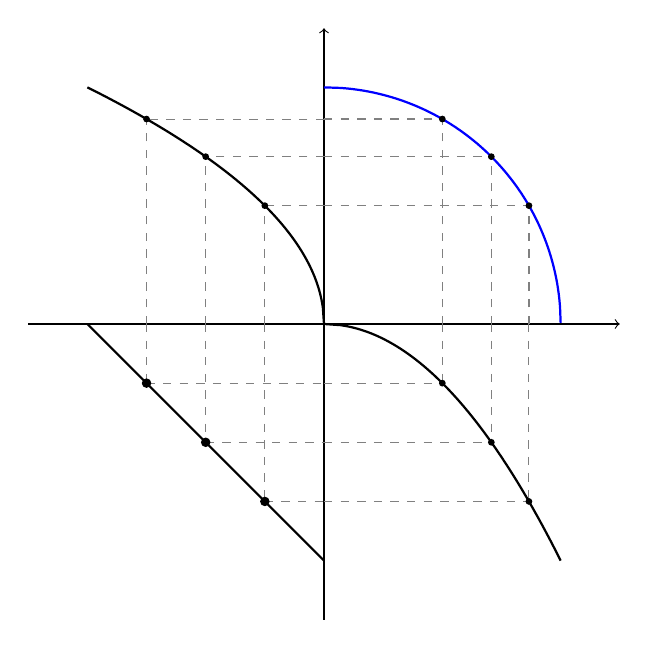
\begin{tikzpicture}
\begin{axis}[
    axis lines=middle,
    xmin=-1.25, xmax=1.25,
    ymin=-1.25, ymax=1.25,
%    xlabel={\small Output of cloth / Labor in cloth},
%    ylabel={\small Output of food / Labor in food},
    xtick=\empty,
    ytick=\empty,
    width=12cm,
    height=12cm,
    axis line style={->},
    clip=false,
    enlargelimits=false,
    domain=0.0:1,
    width=0.75\textwidth,
    height=0.75\textwidth,
    samples=200
]

\pgfmathsetmacro{\a}{0.5}       % curvature parameter

% NW: Production function for food (plot in 2nd quadrant)
\addplot[black, thick] ({-x}, {x^(\a)});
%\node[anchor=south west] at (axis cs:-0.6,0.7) {\scriptsize Production function for food};

% SW: Labor allocation AA curve (line in 3rd quadrant)
\addplot[black, thick] ({-x}, {-1 + x});
%\node[anchor=north east] at (axis cs:-0.95,-0.05) {\scriptsize Economy's allocation of labor (AA)};

% SE: Production function for cloth (4th quadrant)
\addplot[black, thick] ({x^(\a)}, {-x});
%\node[anchor=north west] at (axis cs:0.6,-0.6) {\scriptsize Production function for cloth};

% NE: Production Possibility Frontier (PPF)
\addplot[blue, thick] ({x^(\a)}, {(1 - x)^(\a)});
%\node[anchor=south east, blue] at (axis cs:0.6,0.65) {\scriptsize $PP$};

% Add points and dashed lines for three allocations
\foreach \x in {0.25, 0.5, 0.75} {
    % Points on AA
    \addplot[mark=*, only marks, mark size=1.5pt] coordinates {({-\x}, {-1 + \x})};
    \addplot[dashed, gray] coordinates {({-\x}, {-1 + \x}) (0, {-1 + \x})};

    % Project to NW (Food PF)
    \addplot[dashed, gray] coordinates {({-\x}, 0) ({-\x}, {\x^(\a)})};
    \addplot[dashed, gray] coordinates {(0, {\x^(\a)}) ({-\x},{\x^(\a)})};
    \addplot[mark=*, only marks, mark size=1pt] coordinates {({-\x}, {\x^(\a)})};
    \addplot[dashed, gray] coordinates {({-\x}, 0) ({-\x}, {-(1-\x)})};

    % Project to SE (Cloth PF)
    \addplot[dashed, gray] coordinates {(0, {-\x}) ({\x^(\a)}, {-\x})};
    \addplot[dashed, gray] coordinates {({\x^(\a)}, 0) ({\x^(\a)}, {-\x})};
    \addplot[mark=*, only marks, mark size=1pt] coordinates {({\x^(\a)}, {-\x})};

    % Project to NE (PPF)
    \pgfmathsetmacro{\Qc}{\x^(\a)}
    \pgfmathsetmacro{\Qf}{(1 - \x)^(\a)}
    \addplot[mark=*, only marks, mark size=1pt] coordinates {(\Qc, \Qf)};
    \addplot[dashed, gray] coordinates {(\Qc, 0) (\Qc, \Qf)};
    \addplot[dashed, gray] coordinates {(0, \Qf) (\Qc, \Qf)};
}


\end{axis}
\end{tikzpicture}
\end{frame}



\begin{frame}{Last Class: Autarky Equilibrium}

\begin{figure}[htbp!]

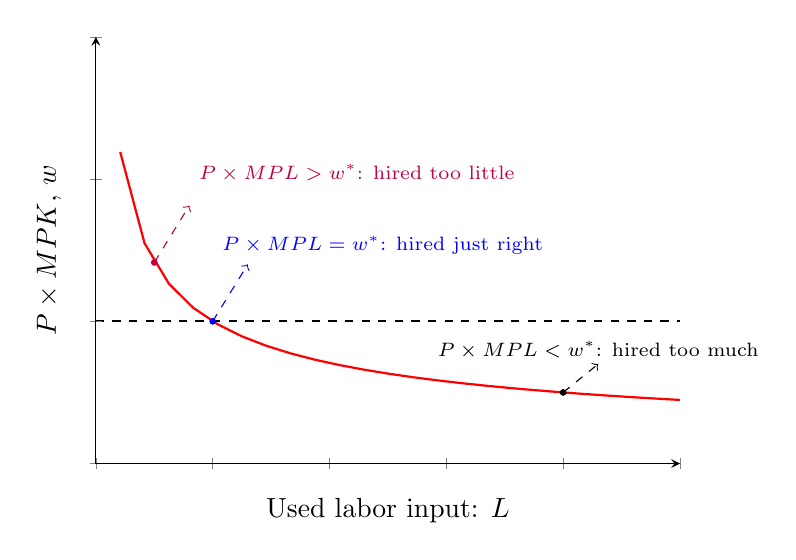
\begin{tikzpicture}
\pgfmathsetmacro{\alpha}{0.5}    % preference for computers
\pgfmathsetmacro{\K}{1}    % labor endowment
\pgfmathsetmacro{\A}{1}    % labor endowment

\centering
\begin{axis}[
    ylabel={$P \times MPK$, $w$ },
    xlabel={Used labor input: $L$},
    ymin=0, ymax=1.5,
    xmin=0, xmax=5,
    yticklabel=\empty,
    xticklabel=\empty,
    axis lines=left,
    enlargelimits=false,
    clip=false,
    axis on top,
    scaled x ticks=false,
    width=9cm, height=7cm,
    title style={font=\bfseries}
]

% PPF: Q_C = (L/a_C) - (a_R/a_C) * Q_R
\addplot[thick, red, domain=0:5] {(1-\alpha)*\A*\K^(\alpha)/x^(\alpha)};


\addplot[dashed, purple, ->] coordinates {(0.5  , {(1-\alpha)*\A*\K^(\alpha)/0.5^(\alpha)}) (0.5 + 0.3, {(1-\alpha)*\A*\K^(\alpha)/0.5^(\alpha)} + 0.2)};
\addplot[mark=*, only marks, purple, mark size=1pt] coordinates {(0.5, {(1-\alpha)*\A*\K^(\alpha)/0.5^(\alpha)})};
\node[anchor=south west, purple] at (axis cs:0.5 + 0.3, {(1-\alpha)*\A*\K^(\alpha)/0.5^(\alpha)} + 0.25) {\scriptsize $P\times MPL > w^*$: hired too little};

\pgfmathsetmacro{\Lb}{((1-\alpha)* \A / 0.5)^(1/\alpha) * \K}    % labor endowment

\addplot[dashed, blue, ->] coordinates {(\Lb, {(1-\alpha)*\A*\K^(\alpha)/\Lb^(\alpha)}) (\Lb + 0.3, {(1-\alpha)*\A*\K^(\alpha)/\Lb^(\alpha)} + 0.2)};
\addplot[mark=*, only marks, blue, mark size=1pt] coordinates {(\Lb, {(1-\alpha)*\A*\K^(\alpha)/\Lb^(\alpha)})};
\node[anchor=south west, blue] at (axis cs:0.5 + 0.5, {(1-\alpha)*\A*\K^(\alpha)/\Lb^(\alpha)} + 0.2) {\scriptsize $P\times MPL = w^*$: hired just right};


\addplot[dashed, black, ->] coordinates {(4  , {(1-\alpha)*\A*\K^(\alpha)/4^(\alpha)}) (4 + 0.3, {(1-\alpha)*\A*\K^(\alpha)/4^(\alpha)} + 0.1)};
\addplot[mark=*, only marks, black, mark size=1pt] coordinates {(4, {(1-\alpha)*\A*\K^(\alpha)/4^(\alpha)})};
\node[black] at (axis cs:4 + 0.3, {(1-\alpha)*\A*\K^(\alpha)/4^(\alpha)}+0.15) {\scriptsize $P\times MPL < w^*$: hired too much};


\addplot[thick, dashed, domain=0:5] {0.5};

\end{axis}

\end{tikzpicture}

\caption{Autarky equilibrium}\label{fig: autarky-num}

\end{figure}
\end{frame}



\begin{frame}{Last Class: Autarky Equilibrium}

\begin{figure}[htbp!]

\begin{tikzpicture}
\pgfmathsetmacro{\alpha}{1/3}    % preference for computers
\pgfmathsetmacro{\K}{1}    % labor endowment
\pgfmathsetmacro{\A}{1}    % labor endowment

\centering
\begin{axis}[
    ylabel={$Y = A \times K^{1/3} L^{2/3}$ },
    xlabel={Used labor input: $L$},
    ymin=0, ymax=5,
    xmin=0, xmax=5,
    yticklabel=\empty,
    xticklabel=\empty,
    axis lines=left,
    enlargelimits=false,
    clip=false,
    axis on top,
    scaled x ticks=false,
    width=9cm, height=7cm,
    title style={font=\bfseries}
]

% PPF: Q_C = (L/a_C) - (a_R/a_C) * Q_R
\addplot[thick, red, domain=0:4] {\A*\K^(\alpha)*x^(1-\alpha)};

\addplot[dashed, gray] coordinates {(0,{\A*\K^(\alpha)*1^(1-\alpha)}) (1,{\A*\K^(\alpha)*1^(1-\alpha)})};
\addplot[dashed, gray] coordinates {(1,{\A*\K^(\alpha)*1^(1-\alpha)}) ({\A*\K^(\alpha)*1^(1-\alpha)},0) };
\addplot[mark=*, only marks, black, mark size=1pt] coordinates {(1, {\A*\K^(\alpha)*1^(1-\alpha)} )};

\addplot[dashed, gray] coordinates {(0,{\A*\K^(\alpha)*2^(1-\alpha)}) (2,{\A*\K^(\alpha)*2^(1-\alpha)})};
\addplot[dashed, gray] coordinates {(2,{\A*\K^(\alpha)*2^(1-\alpha)}) (2,0)};

\addplot[mark=*, only marks, black, mark size=1pt] coordinates {(2, {\A*\K^(\alpha)*2^(1-\alpha)} )};

\addplot[dashed, gray] coordinates {(0,{\A*\K^(\alpha)*3^(1-\alpha)}) (3,{\A*\K^(\alpha)*3^(1-\alpha)})};
\addplot[dashed, gray] coordinates {(3,{\A*\K^(\alpha)*3^(1-\alpha)}) (3,0)};
\addplot[mark=*, only marks, black, mark size=1pt] coordinates {(3, {\A*\K^(\alpha)*3^(1-\alpha)} )};

\addplot[dashed, gray] coordinates {(0,{\A*\K^(\alpha)*4^(1-\alpha)}) (4,{\A*\K^(\alpha)*4^(1-\alpha)})};
\addplot[dashed, gray] coordinates {(4,{\A*\K^(\alpha)*4^(1-\alpha)}) (4,0)};
\addplot[mark=*, only marks, black, mark size=1pt] coordinates {(4, {\A*\K^(\alpha)*4^(1-\alpha)} )};

\end{axis}

\end{tikzpicture}

\caption{Autarky equilibrium}\label{fig: autarky-num}

\end{figure}
\end{frame}


\begin{frame}{Last Class: Autarky Equilibrium}

\begin{figure}[htbp!]

\begin{tikzpicture}
\pgfmathsetmacro{\alpha}{2/3}    % preference for computers
\pgfmathsetmacro{\K}{1}    % labor endowment
\pgfmathsetmacro{\A}{1}    % labor endowment

\centering
\begin{axis}[
    ylabel={$Y = A \times K^{1/3} L^{2/3}$ },
    xlabel={Used labor input: $K$},
    ymin=0, ymax=5,
    xmin=0, xmax=5,
    yticklabel=\empty,
    xticklabel=\empty,
    axis lines=left,
    enlargelimits=false,
    clip=false,
    axis on top,
    scaled x ticks=false,
    width=9cm, height=7cm,
    title style={font=\bfseries}
]

% PPF: Q_C = (L/a_C) - (a_R/a_C) * Q_R
\addplot[thick, red, domain=0:4] {\A*\K^(\alpha)*x^(1-\alpha)};

\addplot[dashed, gray] coordinates {(0,{\A*\K^(\alpha)*1^(1-\alpha)}) (1,{\A*\K^(\alpha)*1^(1-\alpha)})};
\addplot[dashed, gray] coordinates {(1,{\A*\K^(\alpha)*1^(1-\alpha)}) ({\A*\K^(\alpha)*1^(1-\alpha)},0) };
\addplot[mark=*, only marks, black, mark size=1pt] coordinates {(1, {\A*\K^(\alpha)*1^(1-\alpha)} )};

\addplot[dashed, gray] coordinates {(0,{\A*\K^(\alpha)*2^(1-\alpha)}) (2,{\A*\K^(\alpha)*2^(1-\alpha)})};
\addplot[dashed, gray] coordinates {(2,{\A*\K^(\alpha)*2^(1-\alpha)}) (2,0)};

\addplot[mark=*, only marks, black, mark size=1pt] coordinates {(2, {\A*\K^(\alpha)*2^(1-\alpha)} )};

\addplot[dashed, gray] coordinates {(0,{\A*\K^(\alpha)*3^(1-\alpha)}) (3,{\A*\K^(\alpha)*3^(1-\alpha)})};
\addplot[dashed, gray] coordinates {(3,{\A*\K^(\alpha)*3^(1-\alpha)}) (3,0)};
\addplot[mark=*, only marks, black, mark size=1pt] coordinates {(3, {\A*\K^(\alpha)*3^(1-\alpha)} )};

\addplot[dashed, gray] coordinates {(0,{\A*\K^(\alpha)*4^(1-\alpha)}) (4,{\A*\K^(\alpha)*4^(1-\alpha)})};
\addplot[dashed, gray] coordinates {(4,{\A*\K^(\alpha)*4^(1-\alpha)}) (4,0)};
\addplot[mark=*, only marks, black, mark size=1pt] coordinates {(4, {\A*\K^(\alpha)*4^(1-\alpha)} )};

\end{axis}

\end{tikzpicture}

\caption{Autarky equilibrium}\label{fig: autarky-num}

\end{figure}
\end{frame}



\end{document}


